\documentclass[lettersize,journal]{IEEEtran}
\usepackage{amsmath,amsfonts}
\usepackage{algorithmic}
\usepackage{algorithm}
\usepackage{array}
\usepackage[caption=false,font=normalsize,labelfont=sf,textfont=sf]{subfig}
\usepackage{textcomp}
\usepackage{stfloats}
\usepackage{url}
\usepackage{verbatim}
\usepackage{graphicx}
\usepackage{cite}

\newcommand{\new}[1]{\textcolor{black}{#1}}
\newcommand{\rev}[1]{\textcolor{blue}{#1}}
\newcommand{\EE}{\text{E}}
\newcommand{\HD}{\text{HD}}



\usepackage{epstopdf}
\usepackage{lineno}
\usepackage{amsthm}

\usepackage{multirow}

\usepackage{booktabs} \usepackage{csquotes}

\usepackage{amsmath}
\usepackage{amssymb}
\usepackage{setspace}
\usepackage{graphicx} 
\hyphenation{methods}

\usepackage{csquotes}
\usepackage{mathtools}
\usepackage{algorithm}
\usepackage{algorithmic}
\usepackage{caption}
\usepackage{thmtools,thm-restate}
\usepackage{url}

\usepackage{xcolor}


\newcommand{\prob}[1]{\Pr\left(#1\right)}
\newcommand{\oneonerlsone}{$(1+1)~\text{RLS}$}
\newcommand{\oneoneIA}{$(1+1)$~IA}
\newcommand{\oneoneOPTIA}{$(1+1)$~Opt-IA}
\newcommand{\jumpcliff}{\textsc{JumpCliff}~}
\newcommand{\cliff}{\textsc{Cliff}$_d$}
\newcommand{\onemax}{\textsc{OneMax}}
\newcommand{\leadingones}{\textsc{LeadingOnes}}
\newcommand{\twomax}{\textsc{TwoMax}}
\newcommand{\trunmax}{\textsc{TruncatedTwoMax}}
\newcommand{\jump}{\textsc{Jump}$_k$}
\newcommand{\linHD}{M$_{\text{linHD}}$}
\newcommand{\expoF}{M$_{\text{expoF(x)}}$}
\newcommand{\expoHD}{M$_{\text{expoHD}}$}
\newcommand\T{\rule{0pt}{2.6ex}}      
\newcommand\B{\rule[-1.2ex]{0pt}{0pt}}

\newcommand{\fastea}{$(1+1)$Fast EA}
\newcommand{\blin}{$\beta_{\text{linHD}}$}
\newcommand{\bexpo}{$\beta_{\text{expoHD}}$}
\newcommand{\Sbexpo}{Symmetric $\beta_{\text{expoHD}}$}

\newcommand{\IPHfcm}{IPH}

\newcommand{\firstBest}{$(1+1)$~Opt-IA$_{\textsc{FirstBest}}$}

\newcommand{\lastBest}{$(1+1)$~Opt-IA$_{\textsc{LastBest}}$}



\newcommand{\RestateCounter}[2]{\setcounter{#1}{\numexpr\getrefnumber{#2}-1\relax}}

\newtheorem{theorem}{Theorem}
\newtheorem{corollary}{Corollary}
\newtheorem{property}{Property}
\newtheorem{lemma}{Lemma}
\newtheorem{definition}{Definition}


\usepackage{refcount}
\hyphenation{a-na-ly-sis}
\hyphenation{Leading-Ones}
\hyphenation{ge-ne-ration}
\hyphenation{ge-ne-rations}
\hyphenation{cha-racte-ris-tics} \begin{document}

\title{Effective Inversely Proportional Hypermutations for Unimodal and Multimodal Optimisation}

\author{IEEE Publication Technology,~\IEEEmembership{Staff,~IEEE,}	

}
\author{Anonymous authors	

}

\markboth{Journal of \LaTeX\ Class Files,~Vol.~14, No.~8, August~2021}{Shell \MakeLowercase{\textit{et al.}}: A Sample Article Using IEEEtran.cls for IEEE Journals}


\maketitle

\begin{abstract}

Artificial Immune Systems (AIS) employing hypermutations with linear static mutation potential have recently been shown to be very effective at escaping local optima of combinatorial optimisation problems at the expense of being slower during the exploitation phase compared to standard evolutionary algorithms.
In this paper, we examine the more commonly used dynamic inversely proportional  hypermutations (IPH) with mutation potential for which previous theoretical analyses have shown disappointing performance. We first show that considerable speed-ups
in hillclimbing phases may be achieved compared to static hypermutations in the ideal situation where the optimum is known if the mutation rates decrease appropriately with either the fitness or the distance to the optimum. Afterwards, we define a simple (1+1)~Opt-IA that uses IPH and ageing for realistic applications where optimal solutions are unknown. The aim of this AIS is to approximate the ideal behaviour of the IPH better and better as the search space is explored and local optima of higher quality are identified.
We present two variants, one that decreases the mutation rate proportionally until the local (global) optimum is identified, and another where the mutation rate may increase again when detecting that the algorithm is stuck on a large plateau of local optima.
We show that the latter variant outperforms standard bit mutations by escaping the local optima on a multimodal function from the literature and that both variants outperform static hypermutations by escaping the local optima of the standard \textsc{Cliff} benchmark function by accepting solutions of lower fitness.  
\end{abstract}

\begin{IEEEkeywords}
Artificial immune systems, heavy-tailed mutations, inversely proportional hypermutations, theory, runtime analysis
\end{IEEEkeywords}

\section{Introduction}
Three recent hot topics in the theory of randomised search heuristics for optimisation in general and in artificial intelligence in particular have been the benefits of mutation operators with higher mutation rates than traditionally employed\cite{FQWGECCO18,FGQWPPSN18,CorusOlivetoYazdani2021TEVC,DoerrGECCO2017FastGA} (or standard operators using higher parameter values than those previously recommended\cite{CorusOlivetoTEVCsteadyGA2017,JumpTEVC2017,CorusOlivetoGecco2019,OlivetoSudholtWitt2020,DoerrDoerrEbel2015,LenglerTEVC2019}), the automatic adaptation of the mutation rate \cite{DoerrDoerrBookChapter,DLOW2018,DoerrEtAl2016B,LissovoiEtAl2020ECJ,LOWAAAI2020} and the analysis of when non-elitist search heuristics are beneficial compared to elitist ones \cite{OlivetoPaizJorgeSudholt2017Algorithmica,LOW2023,Lehr2021AAAI,DoerrComma2020,CaseLehreTEVC,DangJansenLehreGECCO2015,DangLehreFOGA2015,LenglerSchillerSieberling2024,HeviaSudholtAlgo24}. 

Artificial Immune Systems (AIS) are a class of bio-inspired algorithms which naturally use both high mutation rates via so-called hypermutation operators, often automatically adapt the mutation rate,  and use non-elitism implicitly through the use of ageing operators, characteristics that are typical in the immune system of vertebrates from which AIS draw inspiration. In this paper we analyse the performance of an adaptive mutation operator called Inversely Proportional Hypermutation (IPH) that aims to increase the mutation rate with (an estimate of) the distance from the optimum, and propose a considerably improved one for efficient unimodal and multimodal optimisation.

AIS for optimisation \cite{DeCastroTimmisBook,MO2020AAAI} are generally inspired by the clonal selection principle  \cite{Burnet1959}.
For this reason they are also often referred  to as {\it clonal selection} algorithms \cite{DeCastroTimmisBook}. 
Clonal selection algorithms are also \rev{popular} in evolutionary multi-objective optimisation~\cite{CoelloEMO2025,Coello2022,COY25,HuangZhou2020,EMOReview}. 
In the literature two key features of clonal selection algorithms have been identified \cite{Brownlee2007}: 
\begin{enumerate}
	\item  The proliferation rate of each immune cell is proportional to its affinity \new{(similarity)} with the selective antigen \new{(pathogen)}: the higher the affinity, 
	the higher the number of offspring generated (clonal selection and expansion). \item The mutation suffered by each immune cell during reproduction is inversely proportional to the affinity of the cell receptor with the antigen: the higher the affinity, 
	the smaller the mutation (affinity maturation).
\end{enumerate}
Indeed, well-known clonal selection algorithms employ mutation operators applied to immune cells (i.e., candidate solutions) with a rate that decreases with their similarity to the 
antigen (i.e., global optima) during affinity maturation. Often such operators are referred to as {\it inversely proportional hypermutations} (IPH). 
\new{Two of the most popular} clonal selection algorithms, Clonalg \cite{DecastroVonzuben2002}   and \new{the} Opt-IA \new{immune algorithm~\cite{CutelloNicosiaPavoneTimmis2007} (as well as their many variants~\cite{ClonalSelectionReview}) both employ inversely proportional hypermutations}.  
The ideal behaviour of the IPH operator is that the mutation rate is minimal in proximity of the global optimum and increases as the difference between the fitness of the global optimum
and that of the candidate solution increases. However, achieving such behaviour in practice may be problematic because the fitness of the global optimum is usually unknown.
As a result, in practical applications information about the problem is used to \new{find} bounds on (or estimates of)  the value of the global optimum\footnote{Alternatively, the fitness of the best candidate solution is sometimes used and 
	the mutation rate of the rest of the population is inversely proportional to the best.}.
Thus, the closer the estimate \rev{is} to the actual value of the global optimum, the closer should the behaviour of the IPH operator be to the desired one.
On the other hand,  if the bound is much higher (e.g., for a maximisation problem)  than the true value, then there is a risk that the mutation rate is too high in proximity of the global optimum 
i.e., the algorithm will struggle to identify the optimum. 

While decreasing the step size as the optimum is approached is \rev{a} common practice in continuous optimisation~\cite{AugerDoerrBook}, previous theoretical analyses for combinatorial optimisation, though, have highlighted various problems with IPH operators from the literature even when the fitness value of the global optimum is known.
Zarges~ \cite{Zarges2008} analysed the effects of mutating candidate solutions with a rate that is inversely proportional to their fitness for the \textsc{OneMax} problem.
She considered two different rates for the decrease of the mutation rate as the fitness increases: a linear decay (i.e., each bit \new{is flipped} with probability $\frac{\textsc{{\color{black}\text{Opt}-}OneMax(x)}}{\textsc{Opt}}$, where \textsc{Opt} is the value of the optimum) 
and an exponential decay (i.e., each bit flips with probability $e^{- \rho \frac{\textsc{OneMax(x)}}{\textsc{Opt}}}$ where $\rho$ is called the {\it decay} parameter).
The motivation behind these choices are that the former operator flips in expectation exactly the number of bits that maximises the probability of reaching the optimum in the next step while the latter is the
operator used in the Clonalg algorithm.  
She showed that if the optimum of \textsc{OneMax} is known, then an algorithm employing such mutation operator\new{s} will require exponential time to optimise \textsc{OneMax} with overwhelming probability (w.o.p.)
in both cases of linear or exponential decays of the mutation rate.
The reason is that the initial random solutions that have roughly half the fitness (i.e., $n/2$) of the global optimum (i.e., $n$) have very high mutation rates. Such rates do not allow the algorithm to make any progress with any reasonable probability even if the decay parameter $\rho$ is chosen very carefully (i.e., $\rho = \ln n$ leads to reasonable mutation rates between $1/n$ and $1/2$ during the optimisation of \textsc{OneMax}).
Hence, the behaviour of the mutation operator leads to very inefficient performance even for the simple OneMax function when the optimum is assumed to be known. 

On the other hand, the Opt-IA clonal selection algorithm, that \new{uses a mutation operator called 'hypermutations with mutation potential'} which also has very high mutation rates has been proven to be efficient by employing a selection strategy called {\it stop at first constructive mutation} (FCM). The strategy evaluates the fitness after each bit is flipped and interrupts the hypermutation immediately if an improvement is detected. \new {Otherwise it returns the bit-string obtained after it has flipped the maximum number of  bits it is allowed to flip i.e., the mutation potential.} 
Indeed, the operator using a static mutation potential (i.e., a linear number of bits are flipped unless an improvement is found along the way) has been proven to be very effective at escaping local
optima of standard multimodal benchmark functions \cite{CorusOlivetoYazdani2019TCS} and at finding arbitrarily good approximations for the Number Partitioning NP-Hard problem \cite{CorusOlivetoYazdaniPPSN2018Approx,CorusOlivetoYazdaniAIJ2019} at the expense
of being slower at hillclimbing during the exploitation phases \rev{-} it is up to a linear factor slower than the standard bit mutation (SBM) used by evolutionary algorithms for easy unimodal functions such as OneMax and LeadingOnes.
Hence, \new{the first insight we provide in this paper is that,} differently from other clonal selection algorithms (such as Clonalg and Opt-IA without FCM), hypermutations with mutation potential coupled with FCM can cope with the desired behaviour of inversely proportional mutation rates by being capable of making progress efficiently with high mutation rates. 
In this paper we first consider whether Opt-IA may become faster during the exploitation phases if inversely proportional mutation potentials are applied rather than static ones.
\new{The reason to believe this is that the hypermutations waste many fitness function evaluations during exploitation, since the probability of flipping bits that lead to an improvement decreases when the optimum is approached.} 
Hence, with high probability the operator flips wrong bits at the beginning of a hypermutation and ends up wasting a linear number
of fitness function evaluations in each hypermutation. On the other hand, if the mutation potential decreases as the optimum is approached, 
then the amount of wasted evaluations should decrease accordingly.

A previous runtime analysis for OneMax of the inversely proportional hypermutations with mutation potential used by Opt-IA~\cite{JansenZarges2011} has shown that the mutation rate is always in the range $[(c/2)n, cn]$ where $M=cn$ is the highest mutation potential. Hence it does not decrease proportionally with the decrease in distance to the optimum as desired and, as a result, no asymptotic speed-ups are achieved compared to static mutation potentials. 

In this paper we first show that considerable speed-ups in \new{hillclimbing} phases may be achieved compared to static hypermutations, 
if the mutation rates decrease appropriately with either the fitness or the distance to the optimum. 
To show this, we analyse the IPH operators for standard unimodal benchmark functions where the performance of static mutation potentials is well-understood~\cite{CorusOlivetoYazdani2019TCS}.
We first identify what speed-ups may be hoped for by analysing the operators in the ideal situation where the location of the optimum is known.
A result of this first analysis is that a mutation potential that increases exponentially with the Hamming distance to the optimum provides the larger speed-ups \new{for hillclimbing unimodal functions}. Furthermore, using the Hamming distance rather than the fitness as the measure to quantify proximity to the optimum
makes the operator robust to fitness function scaling.
\new{However, an exponential decay with the distance to the optimum also implies that high mutation rates would occur only when the current solution is prohibitively far away from the optimum, \rev{thus, the algorithm would flip just one bit most of the time, i.e., very rare hyper-mutations}. For instance, a randomly generated solution with expected Hamming distance $n/2$ from the optimum flips $\sqrt{n}$ bits and this mutation will decrease exponentially fast with further improvements. For this reason we find that a linear decrease of the mutation rate is a better compromise in \rev{practice} as it allows for longer phases where large mutations occur} \textcolor{black}{ and it flips the number of bits that increase the probability of hitting the optimum in the next step.}




\begin{table*}[t!]
	\caption{Expected runtimes of the different mutation operators when embedded in a (1+1) algorithmic framework for the benchmark functions considered in this paper. For all results the optimum is unknown to the algorithms. \rev{The $*$ indicates that we do not find it worth the effort to perform a formal analysis, yet for reasons provided at the end of Section~\ref{sec:ltj}, the upper bound is correct.} 
	$\beta:= \log_2 \frac{20}{c}$\textcolor{blue}{, where $c\le 1$ is the constant factor in the \linHD\ potential $M = \lfloor c\cdot H(x,\mathit{best})\rfloor$}.
	}
\begin{center}
	\resizebox{2\columnwidth}{!}{
		
		\begin{tabular}{ |l l l l l| }
			\hline
			(1+1) Algorithms & \textsc{OneMax} &  \textsc{LeadingOnes} & \textsc{Cliff}$_d$ &\textsc{LeadingTrapJump}$_k,\rho$
			\T\B \\ \hline
			
			EA  (SBM) &$\Theta(n \log n)$ \cite{DrosteJansenWegener2002}& $\Theta(n^2)$ \cite{DrosteJansenWegener2002} & $\Theta(n^d)$ \cite{JaegerskuepperStorch} & \color{black}{$n^{\Omega(\log n)}$}
			\T\B\\
			
			
			Opt-IA$_{\textsc{static}}$ & $\Theta(n^2\log n)$ \cite{CorusOlivetoYazdani2019TCS} & $\Theta(n^3)$\cite{CorusOlivetoYazdani2019TCS} &$O(\frac{n^{d+1}\cdot e^d}{d^d})$ \cite{CorusOlivetoYazdani2019TCS} & \color{black}{$O(n\tau + n^{2k+3} + n^{\beta+1})^*$}
			\T\B\\
			
			
			
			Opt-IA$_{\textsc{LastBest}}$ & $\Theta(n \log n) $ & $\Theta(n^2)$& \color{black}{$O\left(\frac{n^{4}\log(n/d)}{d^{2}} + n^{2}\log d\right)$} & \color{black}{$2^{\Omega(n)}$}			\T\B \\
			Opt-IA$_{\textsc{FirstBest}}$ & $\Theta(n \log n)$ & $\Theta(n^3)$ &$O\left(\frac{n^{5}\log(n/d)}{d^{3}} + n^{2}\log d\right)$&    $O(n\tau + n^{2k+3} + n^{\beta+1})$
			\T\B \\

			\hline
		\end{tabular}
	}
	
\end{center}
\label{table:summary}
\end{table*}





Afterwards we propose a clonal selection algorithm that we call (1+1)~Opt-IA
that uses IPH and ageing\footnote{The well-known Opt-IA AIS uses both operators in combination~\cite{CutelloNicosiaPavoneTimmis2007}.} \cite{CutelloNicosiaPavoneTimmis2007} to be applied in practical unimodal and multimodal applications where the optimum is not known. 
The algorithm uses the best solution it has encountered to estimate the mutation rates.
In the literature it has been shown that ageing allows algorithms to escape from local optima either by identifying a new slope of increasing fitness or by completely restarting the optimisation process if it cannot escape~\cite{OlivetoSudholt2014ageing,CorusOlivetoYazdaniGECCO2017,CorusOlivetoYazdaniAIJ2019,HorobaJansenZarges09,JansenZarges2011}. 
\new{The idea behind our proposed AIS is that the more the search space is explored, the better is the ideal behaviour of the IPH approximated through the discovery of better and better local optima.
We propose two variants. The first one, called $(1+1)$~Opt-IA$_{\textsc{LastBest}}$, updates the location of the best seen solution whenever a new solution with fitness value at least as good as the previous one is identified. This guarantees that the mutation rate is minimal on the optimum once it is identified, exactly in the spirit of inversely proportional hypermutations, and allows for the best possible expected runtimes when hillclimbing unimodal functions such as \textsc{OneMax} and \textsc{LeadingOnes}. However, the Opt-IA using such an operator loses power compared to static hypermutations because it cannot escape from the best identified local optima via large mutations as its mutation rate will be minimal. To this end, we define a second variant called $(1+1)$~Opt-IA$_{\textsc{FirstBest}}$, that only updates the location of the best seen solution when a strictly better solution is identified. This algorithm is capable of increasing its mutation rate again when stuck on large plateaus of local optima by increasing its Hamming distance from the best seen solution.
}

\new{We first use the \textsc{Cliff} benchmark function to prove the effectiveness of the IPH over static hypermutations. In particular, we show} 
that the IPH can escape local optima when coupled with ageing, \new{because this operator allows the algorithm to escape the local optimum by accepting solutions of inferior fitness.} We remark that static hypermutations cannot optimise the function efficiently because the operator only stops if a constructive mutation is identified, thus will not return inferior solutions that may survive the ageing operator and allow the algorithm to escape the local optima of the function class. \new{This makes a difference between polynomial and superpolynomial runtimes for super-constant cliff distances, and an expected runtime of $O(n^2 \log n)$ versus exponential for linear cliffs. 
A different problem would occur if hypermutations inversely proportional to fitness were to be used. Since the difference in fitness between the local optima and the bottom of the Cliff is very large, the operator's mutation rate at the bottom of the cliff would be too high leading the algorithm back to the local optima with high probability.}

\new{We conclude the paper by providing an example benchmark function where it is necessary to escape from local optima using large mutations. Thus the $(1+1)$~Opt-IA$_{\textsc{FirstBest}}$ is efficient while traditional standard bit mutations (SBM) that use lower mutation rates are not. The benchmark function, called \textsc{LeadingTrapJump}, is inspired from one previously used in the literature to highlight when high mutation rates are beneficial and when not~\cite{OlivetoLehreNeumann09}. Essentially, by switching the fitness values of the local optima and the global optimum one can provide examples where SBM outperforms high mutation rates and viceversa. Herein we show that the the $(1+1)$~Opt-IA$_{\textsc{FirstBest}}$ can identify the global optimum in both cases.}



A summary of the results obtained in the paper is provided in Table \ref{table:summary} highlighting the speed-ups achieved by the two IPH operators compared to the standard bit mutations traditionally  used by evolutionary algorithms and to the static hypermutation operator with FCM.
\new{It can be noticed how the $(1+1)$~Opt-IA$_{\textsc{FirstBest}}$ is a better compromise to hillclimb faster and allow escaping local optima both by accepting solutions of inferior fitness {\it and} by performing large jumps in the search space making a difference between polynomial and super-polynomial runtimes.}

\new{The original extended abstract~\cite{CorusOlivetoYazdaniIPH2019} of this paper analysed the advantages of using an exponential decay of the mutation rate since this provides the largest speed-ups for unimodal functions in ideal conditions where the optimum is known (see Section \ref{sec:OptKnown}). However, a great disadvantage of the exponential decay is that large mutations hardly ever occur in practice. Indeed no superiority of IPH over a SBM operator was provided.  To this end, in this paper we analyse the use of the linear decay operator and  provide examples where the IPH indeed considerably outperforms SBM providing a difference between polynomial and superpolynomial expected runtimes.}
Due to space restrictions a self-contained paper presenting all proofs is provided as supplementary material.



 
 
 
 \section{Inversely Proportional Mutation Potentials} Hypermutations with mutation potential using FCM flip at most a linear amount of bits (i.e., the mutation potential $M=cn$) chosen uniformly at random without replacement \new{from the interval $[1..n]$}. After each of the $M$ bit flips, the fitness of the produced solution is evaluated and if a {\it constructive mutation} is identified, then the operator is stopped and the solution returned. \new{A  constructive mutation is a solution that is at least as good as that of the original parent.}
 Otherwise the algorithm continues flipping the bits without setting them back until the potential $M$ of bit flips is reached. If no constructive \new{mutation} has been identified earlier, then the $M$-th solution is returned.  
The original inversely proportional hypermutation operator (\IPHfcm{}) proposed for Opt-IA uses mutation potential  $M=\lceil(1-f_{\text{OPT}}/v)cn\rceil $ for minimisation problems, where \textcolor{blue}{$f_{\text{OPT}}\ge 0$ is the optimal fitness value, $v>0$ is the fitness of the current individual,} 
 \new{and $0<c\leq 1$ is some constant}~\cite{CutelloNicosiaPavoneTimmis2007,JansenZarges2011}. 
In an analysis for \rev{$\textsc{ZeroMin}:=n+1-\textsc {OneMax}$}~\cite{JansenZarges2011}, such a mutation potential was shown not to decrease below $cn/2$, with $cn$ being the highest possible mutation potential.
 	As a result no speed-ups at hillclimbing are achieved compared to static hypermutations as the mutation potential is always at least linear.
 In this section, we introduce three different IPH operators  that will be analysed in this paper and that provably speed-up the hillclimbing  performance for \textsc{OneMax}. Two have been already considered in the literature while the third one is newly proposed by us based on analysed drawbacks of the first two at speeding up hillclimbing.
 	 
 \subsection*{Hamming Distance Based Linear Decrease}
 Zarges analysed an inversely proportional hypermutation operator where the probability of flipping each bit increases linearly with the Hamming distance to the optimum or its best available estimate~\cite{Zarges2008}.
Precisely, this operator flips each bit with probability $H(x,\text{best})/n$ where $n$ is the size of the problem and $H(x,\text{best})$ is the Hamming distance of the current point to the best individual (or an estimate if not available). As the expected number of bit-flips is $H(x, \text{best})$ during each execution of a mutation operator, a mutation potential inspired by this inversely proportional hypermutation is:
\begin{align*}M_{\text{linHD}}(x):=H(x,\text{best}).
 \end{align*}
 
\subsection*{Fitness Difference Based Exponential Decrease}
In Clonalg's  IPH,  
 	the mutation probability decreases as an exponential function of the fitness of the current solution~\cite{DecastroVonzuben2002}. Precisely, each bit flips with probability $e^{-\rho \cdot v}$ where $v$ is the normalised fitness value and $\rho$ is a decay parameter that regulates the speed at which the mutation rate  decreases.
 Since we consider maximisation problems, we use $v=\frac{f(x)}{f(\text{best})}$ as suggested by~\cite{Zarges2008} where $f(\text{best})$ is the best known fitness value. Using the expected number of bits flipped by this mutation operator as a mutation potential gives $M=n \cdot e^{-\rho  v}$. According to both experimental and theoretical analyses 
 \cite{Zarges2008}, a reasonable value for $\rho$ is $\ln n$. We call this mutation potential~{\expoF } and define it as:
 \begin{align*} M_{\text{expoF(x)}}(x):=\left\lfloor n^{1-\frac{f(x)}{f(\text{best})}} \right\rfloor.
 \end{align*}
 
 
 \subsection*{Hamming Distance Based Exponential Decrease}
 It is well understood that fitness-proportional selection is sensitive to the difference between the fitness values of candidate solutions, i.e., it struggles to distinguish between solutions that have similar, yet different, fitness values~\cite{OlivetoWittTCS2014,OlivetoWitt2015,Whitley1989,NeumannOlivetoWitt2009}. For this reason, nowadays selection operators that rank individuals by fitness (e.g., tournament, linear ranking, comma selection) are generally preferred. We also consider a measure that  avoids using the fitness values directly because, apart from the above consideration, the ideal amount of bits to be flipped clearly depends on the genotypic distance of the candidate solution to the optimum rather than on their difference in fitness values. To this end, we suggest a mutation potential which is similar to {\expoF } with the exception that it uses the normalised Hamming distance to the best estimate rather than the normalised fitness. We call this mutation potential {\expoHD } and define it as \expoHD$=\lfloor n \cdot e^{-\rho \frac{n-H(x,\text{best})}{n}}\rfloor$ where $n$ is the problem size (the maximum Hamming distance between  any two  points), $H(x,\text{best})$ is the Hamming distance to the best known solution and $\rho$ is the decay of the mutation potential. For the choice of $\rho=\ln n$, we get: \begin{align*}M_{\text{expoHD}}(x):=\left\lfloor n^{\frac{H(x,\text{best})}{n}} \right\rfloor.
 	\end{align*}
 	
 	
\section{Performance Gains in Ideal Conditions}\label{sec:OptKnown} 






In this section, we evaluate the performance of the three different \IPHfcm{} operators, assuming the optimum is known (i.e., best $=$ opt). Under this assumption, the operators exhibit their ideal behaviour (i.e., the mutation potential decreases with the desired rate as the optimum is approached).
Our aim is to evaluate what speed-ups can be achieved in ideal conditions compared to the well-studied static mutation potentials. To achieve such comparisons we perform runtime analyses of the (1+1)~IA  using the \IPHfcm{} on the standard \textsc{OneMax} and \textsc{LeadingOnes} unimodal benchmark functions for which the performance of the same algorithm using static mutation potentials is known~\cite{CorusOlivetoYazdani2019TCS}. The \rev{simple-to-define} \textsc{OneMax} function counts the number of 1-bits in \new{a} bit string and is normally used to evaluate the hill climbing ability of algorithms~\cite{LehrTEVC2018,CorusOlivetoTEVCsteadyGA2017,CorusOlivetoAlgo2020,DoerrDoerrEbel2015}. On the other hand, \textsc{LeadingOnes} is a slightly harder unimodal problem which counts the consecutive number of 1-bits at the beginning of the bit string before the first 0-bit \rev{or the end of the string}. 
Evolutionary algorithms using standard bit mutation (or bit flip local search mutation) optimise the functions respectively in $\Theta(n \log n)$ and $\Theta(n^2)$ expected fitness function evaluations \cite{DrosteJansenWegener2002,BoettcherEtAl2010,DoerrEtAl2016B,LissovoiOlivetoWarwicker2020,DLOW2018}, while static hypermutations are a linear factor slower\cite{CorusOlivetoYazdani2019TCS}.

While in practice both evolutionary algorithms and artificial immune systems use a population of solutions, in this paper we consider single trajectory algorithms to better highlight the performance of all the considered hypermutation operators.
The pseudo-code of a simple AIS,  the (1+1) Immune Algorithm (\oneoneIA{}), is given in Algorithm~\ref{alg:simple}. It simply uses one candidate solution in each iteration to which inversely proportional hypermutations are applied. For the function Hypermutate$(x)$, \IPHfcm{} performs two steps: 
1) it calculates the mutation potential $M$, and 2) it creates $y$ by flipping at most $M$ distinct bits of $x$ selected uniformly at random without replacement one after another until a constructive mutation happens. Otherwise it returns the last constructed solution. A  constructive mutation is a mutation step where the evaluated bit string is at least as fit as the parent \new{$x$}. The pseudo-code of the operator once the mutation potential $M$ has been calculated is depicted in Algorithm~\ref{alg:hypermutate}.
The results proven in this section and comparisons with static hypermutations and the IPH operators from the literature are summarised in Table~\ref{table:afl}.


Before stating the main results, we first introduce two lemmata. The first is the Ballot theorem which is used throughout this paper to derive lower bounds on the expected runtime of the algorithms~\cite{feller1968,JansenZarges2011,CorusOlivetoYazdani2019TCS}.  This theorem is essentially used to show the probability of picking more 1-bits than 0-bits during one hypermutation operation given that there are more 1-bits in the initial bit-string (or vice-versa). 
\begin{lemma} [Ballot Theorem~\cite{feller1968}] \label{lem:ballot} 
In a ballot, suppose that candidate P receives $p$ votes and candidate Q receives $q$ votes such that $p>q$. The probability that throughout the counting P is always ahead of Q is $(p-q)/(p+q)$. 
\end{lemma}

{\color{black}In the context of hypermutation operators, the vote counts are the initial number of $0$ and $1$-bits in the solutions, while counting the votes correspond to flipping them until the first constructive mutation. The probability that a constructive mutation is found is equivalent to the probability of the $Q$ candidate having as many votes counted as the other during any time in the counting process.}

Our second lemma will be used to transform inverse polynomial exponents that arise from the exponential potential.
\begin{lemma}\label{lem:expo}
	For large enough $n$ and {\color{black}any arbitrary constant} $\epsilon$, 
	$n^{1/n^{\epsilon}}= (1+\frac{\ln{n}}{n^{\epsilon}})(1 \pm o(1))$.
\end{lemma}
\begin{proof}
	$n^{\frac{1}{n^\epsilon}} = e^{\frac{\ln(n)}{n^\epsilon}} = 1 + \frac{\ln(n)}{n^\epsilon} + o(\frac{\ln(n)}{n^\epsilon})$ by the Taylor's series of the exponent.
\end{proof}



\begin{table}[t!]
\caption{Comparison of the expected runtimes obtained by different hypermutation schemes for \textsc{OneMax} and \textsc{LeadingOnes}. The original IPH operator of Opt-IA \cite{CutelloNicosiaPavoneTimmis2007}  has the same expected runtimes as the $(1+1)~$IA using static hypermutations \cite{JansenZarges2011}. \new{`$^*$' indicates that the result can be easily drawn from the analysis for \textsc{OneMax} \cite{Zarges2008}.}}
\begin{center}
\resizebox{\columnwidth}{!}{
	\begin{tabular}{ |l l l| }
		\hline
		\oneoneIA & \textsc{OneMax} &  \textsc{LeadingOnes} 
		\T\B \\ \hline
		
		Using static hypermutation & $\Theta(n^2\log n)$  \cite{CorusOlivetoYazdani2019TCS} & $\Theta(n^3)$ \cite{CorusOlivetoYazdani2019TCS}
		\T\B\\
		
		 Clonalg with linear decay & $e^{\Omega(n)}$ \cite{Zarges2008}  & ${e^{\Omega(n)}}^*$
		\T\B\\
		
		 Clonalg with expo decay & $e^{\Omega(n)}$ \cite{Zarges2008}  & ${e^{\Omega(n)}}^*$
		\T\B\\
		
		
		Traditional Opt-IA & $\Theta(n^2 \log n)$ \cite{JansenZarges2011}  & $\Theta(n^3)$ \cite{JansenZarges2011} 
		\T\B\\
		
		FCM with {\linHD } & $\Theta(n^2)$ & $\Theta(n^3)$
		\T\B\\
		FCM with \expoF & \textcolor{blue}{$\Theta(n^{3/2}/\log n)$} & \textcolor{blue}{$\Theta(n^3/\log^2 n)$}
		\T\B \\
		FCM with \expoHD & \textcolor{blue}{$\Theta(n^{3/2}/\log n)$} & \textcolor{blue}{$\Theta(n^{5/2}/\log^2 n)$}
		\T\B \\
		

		\hline
	\end{tabular}
}
\end{center}
\label{table:afl}
\end{table}




\begin{algorithm}[t] 
\caption{\oneoneIA}
\begin{algorithmic}[1] \STATE{Initialise $x \in\{0,1\}^n$ uniformly at random;}
\STATE Evaluate $f(x)$;      
\WHILE{termination condition is not satisfied} {\color{black}
\STATE Update mutation potential $M$;  
\STATE{ $y:=$ Hypermutate$(x, M)$};}
\IF {$f(y) \geq f(x) $}
\STATE{$x:=y$}.
\ENDIF
\ENDWHILE
\end{algorithmic} \label{alg:simple}
\end{algorithm} 

\begin{algorithm}[t]

	\caption{\textsc{Hypermutate}$(x,M)$}
	\begin{algorithmic}[1]
{\color{black}
		\STATE $y \gets x$;
		\FOR{$i = 1$ \textbf{to} $M$}
		\STATE Flip one previously unflipped bit of $y$ chosen uniformly at random;
		\STATE Evaluate $f(y)$;
		\IF{$f(y) \geq f(x)$}        
		\STATE \textbf{return} $y$;
		\ENDIF
		\ENDFOR
		\STATE \textbf{return} $y$;     
	}
	\end{algorithmic}
	\label{alg:hypermutate}
\end{algorithm}


\subsection{Performance for \textsc{OneMax} in Ideal Conditions}
\begin{figure}[t!]
\centering

\includegraphics[width=\columnwidth]{a}
\caption{Static and inversely proportional mutation potentials for \textsc{OneMax}.}
\label{fig:onemax}
\end{figure}

The following theorems derive the expected runtimes using each of the three IPH operators for the function $\textsc{OneMax}(x):=\sum_{i=1}^{n}x_i$. 
Figure \ref{fig:onemax} shows how the studied mutation potentials ideally decrease during the run of the algorithm when optimising the function. 
Notice that for \textsc{OneMax} the behaviours of   {\expoF } and {\expoHD }  are the same. 
By decreasing the potential linearly with the decrease of the Hamming distance, a logarithmic factor may be shaved off from the expected runtime of the {\oneoneIA } compared to the expected runtime achieved by the same algorithm using static hypermutation potentials.



\begin{theorem} \label{th:linHD-OM}
The {\oneoneIA } using \IPHfcm{} with {\linHD } optimises \textsc{OneMax} in $\Theta(n^2)$ expected fitness function evaluations.
\end{theorem}

\begin{proof}
Considering $i$ as the number of 0-bits in the candidate solution, the probability of improvement in the first step is $i/n$. Knowing that at most $n$ improvements are needed to find the optimum and that in case of failure $H(x,\text{opt})=i$ fitness function evaluations would be wasted, the total expected time to optimise \textsc{OneMax} is at most $\sum_{i=1}^n \frac{n}{i} \cdot i =O(n^2)$.

For the lower bound, we use the Ballot theorem (Lemma~\ref{lem:ballot}). 
\new{We flip at most $M \le n$ bits, and the probability that an improvement happens is the probability that at some moment there will be at least as many flipped zeros as there are flipped ones. So pessimistically we can assume that  $M = n$ bits are always flipped, since it maximizes the chances of this unfortunate event.} 

By Chernoff bounds, the number of 0-bits in the initialised solution is at least $n/3$ w.o.p. Considering the number of 
0-bits as $i=q$ and the number of 1-bits as $n-i=p$, the probability of 
an improvement is at most $1-(p-q)/(p+q)=1-(n-2i)/n=\frac{2i}{n}$ by the Ballot theorem, where $i=H(x, opt)$. This means that we need to wait at least $\frac{n}{2i}$ iterations to see an improvement and each time the mutation operator fails to improve the fitness {(\color{black}$\frac{n}{2i} - 1$ times in expectation)}, $i$ fitness function evaluations will be wasted. Considering that at least $n/3$ improvements are needed, the expected time to optimise \textsc{OneMax} is larger than \textcolor{blue}{$(1-2^{-\Omega(n)})\sum_{i=1}^{n/3} {\color{black}\left(\frac{n}{2i}-1\right)} \cdot i = \Omega(n^2)$} \rev{since the operator cannot improve the \textsc{OneMax} function value by more than one in each application due to FCM. The factor $(1-2^{-\Omega(n)})$ accounts for the w.o.p.\ Chernoff event; since $2^{-\Omega(n)}=o(1)$, the bound holds unconditionally}.
\end{proof}

The following theorem shows that a greater speed up may be achieved if the potential decreases exponentially rather than linearly. Note that for \textsc{OneMax} the Hamming distance of a solution to the optimum and its difference in fitness are the same. \new{Hence, there is no difference between the behaviours of the algorithm when using $M_{expoF(x)}$ and $M_{expoHD}$.} 
Figure \ref{fig:onemax} highlights the reason why these operators waste fewer fitness evaluations.




\begin{restatable}{theorem}{expofx} \label{cor:omexpohd}
The {\oneoneIA } using IPH with either {\expoF } or {\expoHD } optimises \textsc{OneMax} in $\Theta(n^{3/2}/\log n)$ expected fitness function evaluations.
\end{restatable}

\textcolor{blue}{The proof is deferred to the supplementary material.}


 


\subsection{Performance for \textsc{LeadingOnes} in Ideal Conditions}
\begin{figure}[t!]
\centering

\includegraphics[width=\columnwidth]{b}
\caption{Static and inversely proportional  mutation potentials for \textsc{LeadingOnes}. Expected values are shown for those using Hamming distance.}
\label{fig:leadingones}
\end{figure}

In the previous subsection, it was shown that decreasing the mutation rate linearly with the Hamming distance to the optimum allows for a logarithmic factor speed-up for \textsc{OneMax} compared to using  static hypermutations. The following theorem shows that no asymptotic improvement over static mutation potentials is achieved for \textsc{LeadingOnes}$:= \sum_{i=1}^{n}\prod_{j=1}^{i}x_i$. The main reason for the lack of improvement is that a linear mutation potential is sustained until at least a linear number of improvements are achieved.


\begin{theorem} \label{th:linHD-LO}
The {\oneoneIA } using \IPHfcm{} with {\linHD } optimises \textsc{LeadingOnes} in $\Theta(n^3)$ expected fitness function evaluations.
\end{theorem}

\textcolor{blue}{The proof is deferred to the supplementary material.}


\rev{We can now proceed with the analysis of the exponential-based potentials.}
Theorem \ref{expohdOnLO} shows that the \rev{fitness difference based exponential}
     mutation potential provides a $\Theta(\log^2 n)$ factor
     speed-up compared to static mutation potentials. 



\begin{theorem} \label{expohdOnLO}
The {\oneoneIA } using \IPHfcm{} with {\expoF } optimises
\textsc{LeadingOnes} in $\Theta(n^3/\log^2 n)$ expected fitness function
evaluations.
\end{theorem}

\textcolor{blue}{The proof is deferred to the supplementary material.}

 

An advantage of Hamming distance-based exponential decays of the mutation potential
compared to fitness-based ones is provided by the following theorem for \textsc{LeadingOnes}.
The reason can be seen in Figure \ref{fig:leadingones}.  While the initial fitness is very low, the potential is very high, but the actual number of bits that have to be flipped to reach the optimum (i.e., the Hamming distance) is much smaller. More precisely, fitness-based potentials suggest to flip $n$ bits when only $n/2$ bits have to be flipped in expectation to reach the optimum in one step. 
{\expoHD } exploits this property, thus wastes fewer fitness evaluations than \expoF. 




\begin{restatable}{theorem}{expohdLO}\label{thm:expohdLO}
The {\oneoneIA } using \IPHfcm{} with {\expoHD } optimises
\textsc{LeadingOnes} in $\Theta(n^{5/2}/\log^2 n)$ expected fitness function
evaluations.
\end{restatable}

\textcolor{blue}{The proof is deferred to the supplementary material.}





 \new{Overall, in this section, we have shown that considerable speed-ups can be achieved in the ideal condition where the optimum is known by using inversely proportional hypermutations compared to static ones.
We conclude} that {\expoHD } provides larger hill-climbing speed-ups compared to the other mutation potentials and is stable to the scaling of fitness functions.
\new{However, {\expoHD } only allows to flip at most $\sqrt{n}$ bits when far away from the optimum (e.g., at initialisation for \textsc{OneMax}), which means that the algorithm hardly ever performs large mutations except at initialisation defeating the purpose of having a hypermutation operator at all. Thus, we believe that \linHD, while being slower during the hillclimbing phases, provides a better balance between high and low mutation rates for hard multimodal functions when the total runtime is reasonably dominated by the time required to escape from local optima. Notice from Table~\ref{table:afl} that using a linear decay operator with FCM  rather than in Clonalg still makes a difference between polynomial and exponential time for the functions when the optimum is known. In the following section we will highlight how being able to perform large mutations more often allows the algorithm to be effective in practice when the optimum is unknown for multimodal functions with very different characteristics.}

 	
 	\section{Behaviour of IPH in Practice}

In this section, we consider the usage of IPH in realistic applications where the optimum is unknown.
 To this end, the mutation rate of the IPH operator will be inversely proportional to the best seen solution rather than to the unknown optimum. 
 
 We combine \IPHfcm{} using {\linHD } with hybrid ageing, as in the Opt-IA AIS \cite{CutelloNicosiaPavoneTimmis2007}, and embed it in a $(1+1)$~Opt-IA shown in Algorithms \ref{alg:alg1+ageing} and \ref{alg:alg2+ageing}. \new{To use \rev{an} ageing operator, an age $\alpha(x)$, is assigned to the individual $x$.} After the Hypermutate$(x)$ operator, the ageing operator is applied.
 	Among the different variants of ageing, {\it hybrid} ageing has been shown to be very efficient at escaping local optima~\cite{OlivetoSudholt2014ageing,CorusOlivetoYazdani2019TCS,CorusOlivetoYazdaniFASTAIS2018,CorusOlivetoYazdaniPPSN2018Approx}. Using this operator,  individuals are assigned with initial age zero. During each iteration of the algorithm, the age  increases by 1 and is passed to the offspring if it does not improve over its parent's fitness. If the offspring is fitter than the parent, then its age is set to 0. At the end of each iteration, any individual with age larger than a threshold $\tau$ is removed with probability \rev{$p_{\text{die}}=1/2$}. In case there is no other individual left, a new individual is initialised uniformly at random\footnote{When a population is used, the required number of individuals are re-initialised to reach the population size again after ageing is applied.}. 
 
 Ageing has been shown to enable algorithms to escape from local optima either by identifying a gradient leading away from it or by restarting the whole optimisation process. Our aim behind the algorithm design is that by escaping local optima via ageing, the number of local optima that are identified by the algorithm increases over time. Thus as time goes by the IPH should approximate its ideal behaviour better and better.
 
\textcolor{black}{Concerning the IPH operator for practical applications we  reintroduce the parameter $c\leq 1$ for determining the mutation potential when it grows linearly with the Hamming distance as in the original Opt-IA~\cite{JansenZarges2011}:}  
 \textcolor{blue}{
 $$M_{\text{linHD}} = \max\!\left(\left\lfloor c \cdot H(x,\mathit{best}) \right\rfloor,\, 1 \right)$$
 }
\textcolor{black}{The parameter will be useful to avoid always ending up in the same basins of attraction as we will see in the analyses of both multimodal function classes we consider in this paper.} 
 
{\color{black} We also have  a design choice regarding the IPH operator  of whether to update the {\it best} seen solution only when a strictly better solution is identified or whether to update it when the algorithm finds a new solution that is as good as the previous best one. 
This design choice leads to considerably different algorithmic behaviours.}
\textcolor{black}{If the current {\it best} is updated to the new solution when individuals of equal fitness are encountered,  then the algorithm will be extremely fast on unimodal functions because the mutation rate will always be the smallest possible (i.e., 1-bit flips). So if the aim is to optimise easy unimodal functions then this version, which we call $(1+1)$~Opt-IA$_{\textsc{LastBest}}$ is the preferred choice, as it can be proved to run in optimal asymptotic runtime on benchmark functions such as \textsc{OneMax} (i.e., $\Theta(n \log n)$) and \textsc{LeadingOnes} (i.e., $\Theta(n^2)$). However, this choice would mean that the algorithm would keep low mutation rates when trapped in the best found local optima if they are encountered again and again with high probability after the algorithm is restarted.}

\textcolor{black}{
The other choice, that of only updating the {\it best} when a strictly better solution is encountered, allows individuals trapped on a large plateau of local optima to increase their \rev{Hamming} distance to the best solution, thus increases the chances of escaping via higher mutation rates. This version, which we call $(1+1)$~Opt-IA$_{\textsc{FirstBest}}$, allows to use high mutation rates more often at the expense of being slower on some unimodal functions like \textsc{LeadingOnes} as we will see. With this operator we remember to update the {\it best} to the last seen \rev{(best)} individual of highest fitness (i.e. the current solution) when ageing is triggered because this limits the \rev{Hamming} distance between the new solution and the current best when a local optima is escaped by accepting solutions of lower fitness, thus decreases the chances of jumping back to the previous local optimum.}
 	
 	
\begin{algorithm}[t] 
 	    \caption{$(1+1)$~Opt-IA$_{\textsc{LastBest}}$ }
     \begin{algorithmic}[1] \STATE{Initialise $x \in\{0,1\}^n$ uniformly at random;} \STATE{set $\alpha(x):=0$ and $\text{best}:=x$};      
 	           \STATE evaluate $f(x)$;    
 	            \WHILE{termination condition is not satisfied} \STATE{$\alpha(x):=\alpha(x)+1$};
\STATE $y:=\text{Hypermutate}(x)$
\IF{$f(y) > f(x)$}
 	            \STATE{$\alpha(y):=0$};
 	            \ELSE
 	            \STATE{$\alpha(y):=\alpha(x)$};
 	            \ENDIF
 	            \IF{ $f(y)\geq f(\text{best})$}
 	            \STATE{ then set $\text{best}:=y$};
 	           \ENDIF
\FOR{$w \in \{x,y\}$}
 	            \IF{$\alpha(w) \geq \tau$}
 	            \STATE with probability $p_{\text{die}}=1/2$:
 	            \STATE \hspace{\algorithmicindent}
 	            reinitialise $w$ uniformly at random,\ $\alpha(w):=0$
 	            \textcolor{blue}{\STATE \hspace{\algorithmicindent}
 	            	\textbf{if} $f(w) \geq f(\text{best})$ \textbf{then}
 	            	\STATE \hspace{2\algorithmicindent}
 	            	$\text{best}:=w$
 	            	\STATE \hspace{\algorithmicindent}
 	            	\textbf{end if}}
 	            \ENDIF
 	            \ENDFOR
 	         \rev{   \IF{$f(y) \geq f(x)$}
 	            \STATE{$x := y$}
 	            \ENDIF}
\ENDWHILE
 	   \end{algorithmic} \label{alg:alg1+ageing}
 	\end{algorithm}
\begin{algorithm}[t] 
 		\caption{$(1+1)$~Opt-IA$_{\textsc{FirstBest}}$ }
 		\begin{algorithmic}[1] \STATE Initialise $x \in\{0,1\}^n$ uniformly at random \STATE set $\alpha(x):=0$ and $\text{best}:=x$      
 			\STATE evaluate $f(x)$    
 			\WHILE{termination condition is not satisfied} \STATE $\alpha(x):=\alpha(x)+1$
 			\STATE $y:=\text{Hypermutate}(x)$
 			\IF{$f(y) > f(x)$}
 			\STATE $\alpha(y):=0$
 			\ELSE
 			\STATE $\alpha(y):=\alpha(x)$
 			\ENDIF
 			\IF{{\color{black}$f(y) > f(\text{best})$}}
 			\STATE $\text{best}:=y$
 			\ENDIF
 			\FOR{$w \in \{x,y\}$}
 			\IF{$\alpha(w) \geq \tau$}
 			\STATE with probability $p_{\text{die}}=1/2$:
 			\STATE \hspace{\algorithmicindent}
 			\textbf{if} $f(w) = f(\text{best})$ \textbf{then}
 			\STATE \hspace{2\algorithmicindent}
 			$\text{best}:=w$
 			\STATE \hspace{\algorithmicindent}
 			\textbf{end if}
 			\STATE \hspace{\algorithmicindent}
 			reinitialise $w$ uniformly at random,\ $\alpha(w):=0$
 			\textcolor{blue}{\STATE \hspace{\algorithmicindent}
 				\textbf{if} $f(w) > f(\text{best})$ \textbf{then}
 				\STATE \hspace{2\algorithmicindent}
 				$\text{best}:=w$
 				\STATE \hspace{\algorithmicindent}
 				\textbf{end if}}
 			\ENDIF
 			\ENDFOR
\rev{ \IF{$f(y) \geq f(x)$}
\STATE{$x := y$}
\ENDIF}
 			\ENDWHILE
 		\end{algorithmic} 
 		\label{alg:alg2+ageing}
 	\end{algorithm}












We start with a general reduction.  When the mutation potential remains~$1$
and ageing is unlikely to trigger, \new{both} algorithm variants execute
single-bit flips with accept-if-$\geq$ and thus behave identically to RLS.
Lemma~\ref{lem:RLS-reduction} below formalises this observation;
we then apply it to show that \new{both} algorithms optimise
\textsc{OneMax} in $\Theta(n\log n)$ and that \lastBest{} optimises
\textsc{LeadingOnes} in $\Theta(n^2)$.

\begin{lemma}[RLS Reduction]\label{lem:RLS-reduction}
Let $A$ denote the event that ageing triggers before the optimum is found
and set $p:=\Pr[A]$.
If \emph{(i)}~$M=1$ throughout every run in which $A$ does not occur, and
\emph{(ii)}~$p=o(1)$ and $\tau p=o(1)$,
then $\mathbf{E}[T']=(1\pm o(1))\,T_{\mathrm{RLS}}$,
where $T_{\mathrm{RLS}}$ is the expected runtime of RLS
 on the same function.
\end{lemma}

\textcolor{blue}{The proof is deferred to the supplementary material.}

\begin{theorem}\label{thm:onemaxexpo}
The expected runtime of \firstBest{} and \lastBest{} using \IPHfcm{} with
\linHD{} and any $c\leq 1$ for optimising \textsc{OneMax} is $\Theta(n\log n)$
with $\tau\geq Cn\ln n$ for a sufficiently large constant~$C$.
\end{theorem}
\begin{proof}
Immediately after initialisation $\mathit{best}=x$, so $H(x,\mathit{best})=0$
and $M=c\cdot H=0$; since the potential is at least~$1$ by convention, $M=1$.
On \textsc{OneMax}, every bit flip changes fitness by $\pm 1$, so no neutral
moves exist; every accepted solution strictly improves fitness and triggers
$\mathit{best}\leftarrow x$ in both variants, maintaining $H=0$ and $M=1$
throughout.  Condition~(i) of Lemma~\ref{lem:RLS-reduction} holds.

For~(ii), at any level $k\geq 1$ the improvement probability is $k/n\geq 1/n$,
so the probability of $\tau$ consecutive non-improvements is at most
$(1-1/n)^\tau\leq e^{-\tau/n}\leq e^{-C\ln n}=n^{-C}$.
A union bound over~$n$ levels gives $p:=\Pr[A]\leq n^{1-C}=o(1)$ for $C>1$,
and $\tau\cdot p\leq Cn\ln n\cdot n^{1-C}=Cn^{2-C}\ln n=o(1)$ for $C>2$.
Thus both conditions of Lemma~\ref{lem:RLS-reduction} hold for $C>2$.

By Lemma~\ref{lem:RLS-reduction},
$\mathbf{E}[T']=(1\pm o(1))\,T_{\mathrm{RLS}}$.
Since $T_{\mathrm{RLS}}=\sum_{k=1}^{n}n/k=\Theta(n\log n)$ (lower bound: at
least $n/3$ zeros initially w.o.p.\ by Chernoff, giving
$\sum_{k=1}^{n/3}n/k=\Omega(n\log n)$), the result follows.
\end{proof}



\new{In the following two theorems we show how \lastBest{} achieves a linear
factor speed-up over \firstBest{} for \textsc{LeadingOnes}, because the latter
increases its mutation rate on plateaus of equal fitness before finding each
improvement.}

\begin{theorem}\label{thm:LBleadingones}
The expected runtime of \lastBest{} using \IPHfcm{} with \linHD{} and any
$c\leq 1$ for optimising \textsc{LeadingOnes} is $\Theta(n^2)$ with
$\tau\geq Cn\ln n$ for a sufficiently large constant~$C$.
\end{theorem}
\begin{proof}
Since \lastBest{} accepts equal-or-better solutions \emph{and} updates
$\mathit{best}$ on any acceptance, every accepted move (whether improving or
neutral) restores $H(x,\mathit{best})=0$, so $M=1$ throughout.
Condition~(i) of Lemma~\ref{lem:RLS-reduction} holds.

For~(ii), the improvement probability at every level is exactly $1/n$
(flip the leftmost $0$-bit), so $(1-1/n)^\tau\leq n^{-C}$
and a union bound over $n$ levels gives $p:=\Pr[A]\leq n^{1-C}=o(1)$.
Moreover $\tau\cdot p\leq Cn^{2-C}\ln n=o(1)$ for $C>2$, verifying
condition~(ii).

By Lemma~\ref{lem:RLS-reduction},
$\mathbf{E}[T']=(1\pm o(1))\,T_{\mathrm{RLS}}$.
For RLS on \textsc{LeadingOnes}, the unique improving move at each of the $n$
levels is the leftmost $0$-bit flip, with probability $1/n$; neutral tail
flips are accepted but do not advance the level.  Hence the expected time per
level is $n$ and $T_{\mathrm{RLS}}=n^2$, giving $\mathbf{E}[T']=\Theta(n^2)$.
\end{proof}

\begin{theorem}\label{thm:FBleadingones}
The expected runtime of the \new{$(1+1)$~Opt-IA$_{\textsc{FirstBest}}$}  with {\linHD } \new{and any $c\leq 1$} for optimising
\textsc{LeadingOnes} is $\Theta(n^3)$ with $\tau=\Omega(n^{1+\epsilon})$ for any arbitrary
constant $\epsilon>0$.
\end{theorem}
\begin{proof}

Fix a level~$\ell$ with $n/3\le \ell \textcolor{blue}{<} 2n/3$. For the current individual $x$ with $\mathrm{LO}(x)=\ell$, we have $x_1=\cdots=x_{\ell}=1$ and $x_{\ell+1}=0$, and the remaining $m:=n-\ell-1$ positions form the tail. In each iteration, the first flipped bit is uniformly distributed over $\{1,\dots,n\}$; therefore the probability that the first flip hits the improving bit $\ell+1$ is $1/n$, the probability that it hits the prefix is $\ell/n$, and the probability that it hits the tail is $m/n$. Let $T$ be the iteration on which the improving bit is first hit. Then $T$ is geometrically distributed with parameter~$1/n$, so $\mathbb{E}[T]=n$. Before this improving iteration occurs, \textcolor{blue}{the expected number of tail-first iterations is
$\frac{m}{n-1}(\mathbb{E}[T]-1) = \frac{m(n-1)}{n-1} = m = \Theta(n)$
(using that, conditional on not hitting the improving bit $\ell+1$, the
first flip is uniform over the remaining $n-1$ positions, of which $m$
are tail positions).} Each such iteration flips a uniformly random tail bit. By standard coupon--collector arguments, after $\Theta(n)$ such tail flips \textcolor{blue}{a constant fraction of the $m$ tail positions has been flipped exactly once
with constant probability (since each hypermutation samples bits without
replacement, each position is visited at most once per call).} Thus, with constant probability, the Hamming distance between $x$ and \textcolor{blue}{$\mathit{best}$} is $\Theta(m)=\Theta(n)$, and therefore the IPH mutation potential satisfies $M=\Theta(n)$ at this level.

Consider now a subsequent iteration at the same level while $M\ge \alpha n$ for some constant $\alpha>0$. If the first flip hits the prefix (an event of probability at least $\ell/n\ge 1/3$), then, because mutation proceeds without replacement, the lost prefix bit cannot be repaired within the same iteration. Consequently, no acceptance can occur in that iteration, and the algorithm executes the entire mutation budget $M$, rejecting at the end. Hence the expected number of fitness evaluations in such an iteration is at least $\alpha n$. Since this happens with probability at least $1/3$, the unconditional expected cost of one iteration while $M=\Theta(n)$ is $\Omega(n)$.

The probability that an iteration yields an improvement is exactly $1/n$, because only a first flip that hits position $\ell+1$ increases the \textsc{LeadingOnes} value. Therefore the expected number of iterations required to advance from level $\ell$ to $\ell+1$ is $1/(1/n)=n$. Combining this with the previous observation, the expected number of fitness evaluations spent at level $\ell$ satisfies $\Omega(n)\cdot n=\Omega(n^2)$.
There are $\Theta(n)$ levels $\ell$ in the interval $[n/3,2n/3]$, and each such level contributes $\Omega(n^2)$ expected evaluations. Thus the total expected optimisation time is $\Omega(n^3)$. Finally, stochastic ageing can only increase the number of evaluations and therefore cannot invalidate the lower bound. Since the function has $n$ levels, $1/n$ probability of improvement and $M\leq n$, the expected runtime is bounded from above by $O(n^3)$ as well.


\end{proof}

\textcolor{black}{In this section, we have proven the results for \linHD. Naturally the same \rev{positive} results follow for the \expoHD~ operator which always has at most the same mutation rate or lower.}


 

\section{When IPH Outperforms Too High Mutation Rates}
\begin{figure}
\centering

\includegraphics[width=0.5\textwidth]{cliff_updated}
\caption{\textcolor{blue}{The \textsc{Cliff}$_d$ function for $n=50$, $d=10$.
The local optimum (40 one-bits, fitness~40) and global optimum
(50 one-bits, fitness~40.5) are labelled.}}
\label{fig:cliff}
\end{figure}

\new{ In this section} we show that {\linHD } combined with ageing can efficiently escape from local optima. We will use the well known \cliff{} function for this purpose where static hypermutations are inefficient~\cite{CorusOlivetoYazdani2019TCS}:
\begin{equation} \label{func:cliff}
	\textsc{Cliff}_{d}(x):=\begin{cases}
		\sum_{i=1}^n x_i & \text{if}\; \sum_{i=1}^n x_i \leq n-d, \\
		\sum_{i=1}^n x_i -d+ 1/2 & \text{otherwise.}
	\end{cases}
\end{equation}
The class of \cliff{} functions, illustrated in Figure~\ref{fig:cliff}, is usually used to assess the performance of non-elitist algorithms. It was originally designed as a problem instance where non-elitist EAs outperform elitist EAs~\cite{JaegerskuepperStorch}. This function  has a \textsc{OneMax} slope with length $n-d$ which leads the algorithms towards the local optima. The local optima are followed by a second \textsc{OneMax} slope (of length $d$) of lower fitness which leads to the global optimum. While elitist algorithms need to make a jump of size $d$ to find the global optimum, \rev{some} non-elitist algorithms can easily find the second slope by accepting inferior solutions, and then hillclimb up to the global optimum \cite{LissovoiOlivetoWarwicker2019AAAI,CorusOlivetoYazdani2019TCS,CorusOlivetoYazdani2021TEVC,HeviaSudholtAlgo24,DoerrIJCAI-25}. 
Due to the high mutation rates of static hypermutations, even if they were to escape the local optima of \cliff{} (which is \new{very unlikely} due to FCM and linear mutation potentials), they would still jump back with high probability.  

\textcolor{purple}{Recently {\it fast} AISs have been introduced~\cite{CorusOlivetoYazdani2021TEVC} that simply flip the required number of bits independently according to the mutation potential (rather than sequentially and using FCM) in a similar fashion to power law mutation operators~\cite{DoerrGECCO2017FastGA}. These have been shown to optimise \cliff{} as long as the gap size is linear in expected time $O(n^{5/2} \log n$).
}

Now we show that differently from static hypermutations, {\linHD }
combined with ageing can escape from the local optima of \cliff{} \textcolor{purple}{also for small cliff gaps, and faster than the {\it fast} AISs for sublinear gaps}, 
hence optimises the function efficiently. The condition that $d$ is not prohibitively large is necessary to avoid
that the reinitialised solutions due to ageing have larger fitness than a solution with $n-d+1$ $1$-bits, {\color{black} which would cause the latter to be removed from the population}.
We believe that this assumption is realistic for practical applications. 


 
{
\rev{The following theorem is the main result of this section.}
\begin{theorem}\label{th:expoHD-cliff}
	The \textcolor{black}{\firstBest~with} \linHD\ (factor $c<\tfrac{1+4\varepsilon}{3-4\varepsilon}$) and ageing parameter $\tau=\Omega(n^{1+\epsilon'})$
	optimises \cliff{} with $d<n(\tfrac{1}{4}-\epsilon)$ in expected
	\[
	O\!\Big(\frac{n^{5}\log(n/d)}{d^{3}} \;+\; n^{2}\log d\Big)
	\]
	fitness function evaluations.
\end{theorem}


We now present the proof sketch of our main result on the  \cliff{} function, together with 
all supporting lemmata.  All proofs are deferred to the supplementary materials. The argument proceeds in two 
major stages: (i) obtaining a canonical entry point onto the second slope 
immediately after an ageing event at the cliff-top; and (ii) showing that from 
this configuration the algorithm reaches the optimum without dangerous increases in mutation potential.

For stage (ii) we will use the generalization of Markov's Inequality by Ville~\cite{Doob1953}(Ch.~VII) which will allow us to show that the mutation potential stays bounded with constant probability.
\begin{theorem}[Ville's inequality for nonnegative supermartingales]\label{thm:ville}
	Let $(M_t)_{t\ge 0}$ be a nonnegative supermartingale adapted to $(\mathcal F_t)_{t\ge 0}$. 
	Then for every $a>0$,
	\[
	\Pr\!\big(\sup_{t\ge 0} M_t \ge a\big)\ \le\ \frac{\EE[M_0]}{a}.
	\]
\end{theorem}



To establish the result, we first analyse how the algorithm reaches a highly 
structured ``canonical'' state shortly after ageing triggers at the cliff-top.
At the cliff-top the algorithm cannot improve except by sampling the global 
optimum, and so ageing will eventually be triggered.  The key insight is that 
the iteration of ageing followed by two additional \textcolor{black}{fitness improvements} can place the 
algorithm into a
\textcolor{blue}{canonical
starting configuration on the second slope.
Throughout the \cliff{} analysis we index the successful fitness improvements on
the second slope by $r = r_0, r_0+1, \dots$, and write $\mathrm{HD}(r)$ for
the Hamming distance between the current solution and \emph{best} after $r$
such improvements.
With this notation, the canonical start corresponds to
$r_0 = 2$ (two improvements completed from the cliff bottom)
and $\mathrm{HD}(r_0) = 2$ (the current solution differs from the locked
\emph{best} in exactly two positions).}  The following lemma formalises this.

\begin{lemma}\label{lem:can-start-omega-d3}
	Suppose ageing is triggered at the cliff-top ($d$~zero-bits).  
	The \rev{\firstBest}~with \linHD\ with $c\in(0,1)$ reaches within at most three steps the 
	configuration
	\[
	r_0=2, \qquad \mathrm{HD}(r_0)=2,
	\]
	with probability at least 
	\[
	\frac{3}{256}\left(\frac{d}{n}\right)^3.
	\]
\end{lemma}


The canonical condition $(r_0,\mathrm{HD}(r_0)) =
(2,2)$ means that we begin the drift analysis two successful improvements into
the second slope, at a point differing from the reference in exactly two
bit positions.

Repeated ascents to the cliff-top therefore form a geometric waiting-time 
process.   \rev{It takes at most $\sum_{i=d}^{n}n/i=O(n\log(n/d))$ for RLS to climb the first slope and the mutation potential is at most linear.
} Since each ascent takes $\rev{O}(n^2\log(n/d))$, the 
total time to obtain the canonical start is \new{provided by the following corollary}.

\begin{corollary}
The expected evaluation count until the first occurrence of 
	$(r_0,\mathrm{HD}(r_0)) = (2,2)$ is 
	\[
	O\!\left(\frac{n^{5}\log(n/d)}{d^{3}}\right).
	\]
\end{corollary}


From the canonical starting point, the key difficulty is \new{showing that} the mutation
potential \new{does not increase} too much.  With only few zero-bits remaining, successful
steps on the second slope require flipping one of these rare zeros, whereas each
$1\!\to0$ flip increases the Hamming distance and thus the mutation potential.
If this potential grows too large, hypermutations become long enough that, under
FCM$(\ge)$, they are increasingly likely to wander back to the cliff-top; once
there, the stopping rule causes the process to lock onto the plateau and erase
all progress.  Hence the analysis must show that with constant probability the
mutation potential stays small throughout the entire second-slope climb.  This
requires  controlling tightly how many detrimental flips a hypermutation can
accumulate before recovering to parent-level fitness.  The next lemma provides
the crucial starting point: an exponential tail bound for this damaging prefix.

\begin{lemma}\label{lem:xi-tail}
	\textcolor{blue}{Let the current solution on the second slope have $z\le d$ zero-bits and
	define $p=z/n$.
	Consider a single application of the hypermutation operator; let $\xi_z$ be
	the number of $1\to0$ flips made \emph{within that one hypermutation} before
	the fitness first returns to $\ge$ the parent's fitness (i.e., before the
	first catch-up).}
	Then for all $k\ge1$,
	\[
	\Pr(\xi_z\ge k)\le (2p)^k.
	\]
	Consequently, the probability that the Hamming distance increases by at least 
	$2k$ in a single hypermutation is also at most $(2p)^k$.
\end{lemma}



A whole \emph{phase} consists of all attempts at the same zero-bit count until the 
first success.  
Using the tail bound above, we obtain uniform exponential moment bounds for 
entire phases.

\begin{lemma}\label{lem:phase-mgf}
	Consider a phase at zero-bit count $z$ and let $Y_z$ denote the total 
	Hamming-distance increase from all failed attempts in the phase.  
	Let $\rho = 2d/n$.  
	For all $0<\lambda<\tfrac12\ln\frac{1}{2\rho}$,
	\[
	\mathbb{E}[e^{\lambda Y_z}] 
	\;\le\; 
	\textcolor{blue}{\frac{1-\rho}{1-\rho e^{2\lambda}}
	\;\eqqcolon\; K(\lambda).}
	\]
\end{lemma}



To track the safety of the mutation potential across phases, we introduce a 
linear \emph{buffer} \new{$B_r = \theta r - s_0 - E_r$} capturing the invariant $c\,\mathrm{HD}(r)\le r$.

\begin{lemma}\label{lem:buffer}
	Let successful phases be indexed by $r=r_0,r_0+1,\dots$ and define
	\[
	s_0=\mathrm{HD}(r_0)-r_0, \qquad 
	\theta=\frac{1}{c}-1, \qquad
	E_r=\sum_{j=r_0+1}^{r} Y_{z_j},
	\]
	and $B_r = \theta r - s_0 - E_r$.
	Then for all $r\ge r_0$:
	\begin{enumerate}
		\item 
		$B_r\ge0$ if and only if $c\cdot\mathrm{HD}(r)\le r$;
		\item 
		$B_{r+1}-B_r=\theta-Y_{z_{r+1}}$;
		\item 
		$B_{r_0}=\theta r_0 - s_0$.
	\end{enumerate}
\end{lemma}


Combining \rev{the MGF of the buffer growth} with the buffer update yields an exponential drift 
envelope suitable for applying \textcolor{black}{Ville's inequality for non-negative supermartingales (Theorem~\ref{thm:ville}).}

\begin{lemma}
\label{lem:drift-envelope-global}
	Let $\rho=2d/n$.  
	For any $0<\lambda<\tfrac12\ln\tfrac{1}{2\rho}$ define
	\[
	\textcolor{blue}{\frac{1-\rho}{1-\rho e^{2\lambda}} \;\eqqcolon\; K(\lambda),}
	\qquad 
	\alpha=e^{-\lambda\theta}K(\lambda).
	\]
	Then for all $t\ge0$,
	\[
	\mathbb{E}[e^{-\lambda(B_{t+1}-B_t)}\mid\mathcal{F}_t]\le \alpha.
	\]
\end{lemma}


\new{We now apply Ville's inequality to turn such a drift envelope into a bound on barrier crossing.}


\begin{corollary}
\label{cor:ville-exponential}
	
	If $B_0=b>0$ and there exist $\lambda>0$ and $\alpha<1$ with
	\[
	\mathbb{E}[e^{-\lambda(B_{t+1}-B_t)}\mid\mathcal{F}_t]\le\alpha,
	\]
	then
	\[
	\Pr\!\left(\inf_{t\ge0} B_t \le 0\right) \le e^{-\lambda b}.
	\]
\end{corollary}



To guarantee the drift negativity required above, we identify the admissible 
range of the mutation-potential factor~$c$.

\begin{lemma}\label{lem:c-threshold-instance}
	
	Let $\rho=2d/n$ and $\theta=\frac{1}{c}-1$.  
	Define
	\[
	c_\star(n,d)=\frac{1-\rho}{1+\rho}.
	\]
	If $c<c_\star(n,d)$, then there exists $\lambda>0$ such that
	\[
	e^{-\lambda\theta}K(\lambda) < 1,
	\]
	and hence the buffer satisfies the Ville barrier bound.
\end{lemma}


A uniform instantiation over all permitted~$d$ shows that the feasible~$c$ 
range has a nontrivial lower bound.

\begin{corollary}If $d\le (\tfrac14-\varepsilon)n$, then
	\[
	c_\star(n,d) \;\ge\; \frac{1+4\varepsilon}{3-4\varepsilon} \;\ge\; \tfrac13.
	\]
\end{corollary}
\label{cor:c-floor}



Finally, combining the threshold on $c$ with the initial buffer value at 
$(r_0,\mathrm{HD}(r_0))=(2,2)$ yields a uniform constant bound on the 
probability of avoiding jumping back.

\begin{lemma}
\label{lem:param-constant-c-general}
	If $c<c_\star(n,d)$ and 
	$b=B_{r_0}=\frac{r_0}{c}-\mathrm{HD}(r_0)>0$, 
	then 
	\[
	\Pr\!\left(\inf B_t \le 0\right) \le e^{-\lambda b}
	\]
	for some $\lambda>0$ depending only on $c$ and $d/n$.  
	For fixed~$\varepsilon$, this yields a uniform constant $<1$ independent of 
	$n,d$.
\end{lemma}


Once the mutation potential remains safe throughout, progress on the second 
slope is monotone and its runtime is easily bounded.



\begin{lemma}\label{prop:climb-time}
	
	If $B_t>0$ for all $t$, then the second-slope ascent completes in expected
	\[
	\Theta(n\log d)
	\]
	iterations.  
	If $\tau=\Omega(n^{1+\varepsilon})$, then $\Theta(n\log d)=o(\tau)$.
\end{lemma}



The expected time to reach the canonical start is 
$O(n^{5}\log(n/d)/d^{3})$.  
Once there, with constant probability the buffer remains positive for all 
phases; conditioned on this event, the second-slope ascent costs 
$O(n^{2}\log d)$ evaluations.  
Since the success probability is constant, this remains the unconditional 
expectation.  
Summing the two contributions establishes the main runtime bound.


\textcolor{black}{The analysis for \lastBest~differs only in Lemma~\ref{lem:can-start-omega-d3} and actually yields a $d/n$ factor better probability bound since the mutation potential is $1$ at the cliff-top and thus, creating a solution at the bottom of the cliff is immediately possible when any cliff top individual dies, whereas for \firstBest~to work we have to first accept a neutral mutation to get the mutation potential to $1$, and then mutate into a cliff bottom solution in the next iteration. Consequently the runtime for \lastBest~is  
$O\!\Big(\frac{n^{4}\log(n/d)}{d^{2}} \;+\; n^{2}\log d\Big)$.}

\textcolor{black}{
\begin{corollary}
	The \textcolor{black}{\lastBest~with} \linHD\ \new{(factor $c<\tfrac{1+4\varepsilon}{3-4\varepsilon}$)} and ageing parameter $\tau=\Omega(n^{1+\epsilon'})$
	optimises \cliff{} with $d<n(\tfrac{1}{4}-\epsilon)$ in expected
	\[
	O\!\Big(\frac{\rev{n^{4}}\log(n/d)}{d^{2}} \;+\; n^{2}\log d\Big)
	\]
	fitness function evaluations.
\end{corollary}
}
The following section will highlight the advantages of using \textsc{First-Best} over using \textsc{Last-Best}.
 }
 
 
 
\section{When IPH Outperforms Too Low Mutation Rates}\label{sec:ltj}
\new{In this section we introduce a function class where inversely proportional hypermutations outperform the lower mutation rates of SBM, and the higher mutation rate on local optima of the $(1+1)$~Opt-IA$_{\textsc{FirstBest}}$ will be essential.}
The function class is inspired \rev{by the} one previously used to show the advantages and disadvantages of using high mutation rates in the context of rank-based mutation in population-based algorithms~\cite{OlivetoLehreNeumann09}.
In rank-based mutation algorithms~\cite{RankBasedMutation} each individual has a different mutation rate based on their rank in the population i.e., the best individual has the lowest mutation rate while the worst individual has a very high one.
The \textsc{LeadingTrapJump} function was introduced as an example where the use of high mutation rates is detrimental while low mutation rates are efficient. \new{However, if the locations of the local and global optima are swapped, then the opposite result can be shown (i.e. high mutation rates are effective while low ones are ineffective).}
We have slightly modified the location of the trap compared to~\cite{OlivetoLehreNeumann09} for our objectives. 




Formally, for constants $k\ge1$ and $\rho\in(0.8,0.9)$, let $r := 2k+1$, 
$L := \lfloor\log_2 n\rfloor$, 
$\mathcal{P} := \{\,x : \mathrm{LO}(x)\ge 0.9n\,\}$, 
$\mathcal{B}_k := \{\,0^{r} 1^{(0.9n-r)} *\,\}$, 
and $\mathcal{D}_\rho := \{\,0^{L} * : |x|_1 \ge \rho n\,\}$.
The function $\mathrm{LTJ}_{k,\rho} : \{0,1\}^n \to \mathbb{R}$ is
\[
\mathrm{LTJ}_{k,\rho}(x)
=
\begin{cases}
	0, & x \in \mathcal{P},\\[2pt]
	\mathrm{LO}\bigl(x_{i>r}\bigr)+r, & x \in \mathcal{B}_k,\\[2pt]
	\textcolor{black}{n+1}, & x \in \mathcal{D}_\rho,\\[2pt]
	\mathrm{LO}(x), & \text{otherwise.}
\end{cases}
\]
\textcolor{blue}{Here $x_{i>r}$ denotes the suffix of $x$ at positions $i > r$, i.e.,
$x_{i>r} := (x_{r+1}, x_{r+2}, \dots, x_n)$.}
 \textcolor{blue}{Note that  $r := 2k+1$ is an odd number, as required for the block-jump prefix $0^r1^{(0.9n-r)}*$
to force an even number of bit-flips to reach $\mathcal{B}_k$, which is
the key parameter controlling the per-iteration success probability
$\Theta(n^{-(r+1)}) = \Theta(n^{-(2k+2)})$. We introduce $r$ as shorthand
to avoid writing $2k+1$ in every exponent throughout the proof.}
\begin{figure}[t]
\centering

\includegraphics[width=0.48\textwidth]{ltj_diagram}
\caption{\textcolor{blue}{The \textsc{LeadingTrapJump}$_{k,\rho}$ landscape (schematic,
$n=30$, $k=1$, $\rho=0.85$).
The x-axis is the \textsc{LeadingOnes} level of the current solution.
From the junction~$J$ (end of the main slope), large mutations can reach
either the block-jump slope~$\mathcal{B}_k$ (leading to the local optimum)
or the deep-prefix plateau~$\mathcal{D}_\rho$ (global optimum).
Both off-slope structures have $\mathrm{LO}(x)=0$; their positions on the
y-axis reflect their fitness values, not their \textsc{LeadingOnes} level.}}
\label{fig:ltj}
\end{figure}

The landscape consists of a long LeadingOnes slope rising from fitness 
$\mathrm{LO}(x)$ up to level $0.9n-1$, followed by a large penalised region.  
Two off-slope structures contain the \textcolor{black}{two sets of optima} but are inaccessible to 
standard hill-climbers.  
The set $\mathcal{B}_k$ begins with the prefix $0^{r}1^{(0.9n-r)} *$ and forms a 
short slope, \new{called block-jump slope,} that \textcolor{black}{deterministically increases toward its unique local optimum 
\textcolor{blue}{$0^{r}1^{(0.9n-r)}$}; reaching 
this prefix is therefore equivalent to entering the leading ones path to the local optimum\textcolor{blue}{
$0^{r}1^{(0.9n-r)}$}.}  
In contrast, the set $\mathcal{D}_\rho$ consists of solutions with prefix 
$0^{L} *$ \textcolor{black}{whose suffix has ones-density at least $\rho$} i.e., $\rho n$ ones, and forms a wide 
plateau of globally optimal fitness, \new{which we call  deep-prefix plateau}.  
\textcolor{blue}{Both structures are hidden behind the penalised barrier (illustrated in
Figure~\ref{fig:ltj}), and the only reliable way to reach them is via large
hypermutation events.}  
The junction $J := \{x : \mathrm{LO}(x)=0.9n-1\}$ acts as a central gateway: 
each ageing epoch that restarts the search will, with high probability, ascend 
the LeadingOnes slope back to $J$ before any off-slope structure is encountered.  
From $J$, the \oneoneOPTIA~using \IPHfcm{}~with \linHD~can perform jumps of the 
appropriate magnitude to reach either the entrance of the block-jump slope $\mathcal{B}_k$ or 
the plateau $\mathcal{D}_\rho$ \rev{i.e., via ageing restarts it will eventually find both optima efficiently.} 
\textcolor{black}{On the other hand, algorithms with lower mutation rates, such as those using SBM will with high probability not be able to flip the logarithmic number of bits required to reach the global optimum, thus have a runtime of $n^{\Omega(\log n)}$ with high probability.}

\begin{theorem} \label{thm:main-tau-final}
The  $(1+1)$~Opt-IA$_{\textsc{FirstBest}}$~with ageing threshold $\tau=\Omega(n^{1+\epsilon})$ using  \linHD~with $c<5/8$  identifies both local and global optima of  $\mathrm{LTJ}_{k,\rho}$ in
	$O(n\tau + n^{2k+3} + n^{\beta+1})$ fitness function evaluations	where $\beta := \log_2 \frac{20}{c}$.
\end{theorem}

To establish Theorem~\ref{thm:main-tau-final} we rely on three ingredients.
First, every ageing epoch returns to the junction $J$ with high probability.
Second, an epoch beginning at $J$ performs sufficiently long jumps to reach the beginning of the block-jump slope with probability $\Theta(n^{-(2k+2)})$ per iteration.
Third, an epoch beginning at $J$ performs a logarithmic jump onto the deep-prefix plateau with probability $\Theta(n^{-\beta})$ per iteration.

Since each event corresponds to reaching either the start of a short slope leading deterministically to its optimum (for $\mathcal{B}_k$) or directly a plateau of global optima (for $\mathcal{D}_\rho$), these per-epoch probabilities govern the entire runtime.

We first need to bound from below the probability that the algorithm visits the junction point after restarts in order to later argue that from the junction point both sets of optima will be accessed.

\begin{lemma} \label{lem:junction-first-density-Bk}
	Starting from any random individual, the $(1+1)$~Opt-IA$_{\textsc{FirstBest}}$~using \IPHfcm{}~with \linHD~\textcolor{black}{and $c<5/8$}  reaches the junction $J = \{x : \mathrm{LO}(x)=0.9n-1\}$ before accepting any individual in $\mathcal{B}_k$ or $\mathcal{D}_\rho$ with high probability.
\end{lemma}

Within $n^2$ iterations, the algorithm performs at least $0.9n$ LeadingOnes 
improvements with high probability.  
Before reaching $J$, deep-prefix entrances require flipping the $L$-bit prefix 
to $0^L$, an event whose probability per iteration is at most $(M(x)/n)^L$.  
Since under \linHD\ the mutation potential satisfies $M(x) \le q^\star n$ for 
some constant $q^\star < 1$ (determined solely by $c$ and $\rho$), this becomes 
$(q^\star)^L = n^{-\alpha^\star}$ for $\alpha^\star := \log_2(1/q^\star) > 2$, 
yielding a total probability of $o(1)$ over $n^2$ iterations.
Thus the slope is climbed to $J$ with high probability.



\textcolor{purple}{The following two lemmata will condition throughout on the event that during an ageing epoch the junction $J$ is reached.
This event happens with high probability by Lemma~\ref{lem:junction-first-density-Bk}.}

\begin{lemma} \label{lem:BJO-epoch}
	\textcolor{blue}{Let an ageing epoch reach the junction $J$.} Then, with probability $\new{p_B}=\Omega(\min\{1,\,\tau\,n^{-(2k+2)}\})$, the epoch performs a jump placing the individual at the beginning of the block-jump slope.
\end{lemma}

The suffix of the individual at $J$ is essentially random relative to the best individual stored from the 
previous epoch. 
With high probability their Hamming distance is at least $n/20$, guaranteeing 
\textcolor{black}{$M(x)= cn/20$} throughout the epoch.  
Under this event, the probability that the first $r+1$ flips of the hypermutation hit exactly the positions defining the prefix $0^{r}1^{(0.9n-r)} *$ is $\Theta(n^{-(r+1)})$.
Evaluating this over $\tau$ iterations yields the stated bound.





\begin{lemma} \label{lem:DPO-epoch}
	\textcolor{blue}{Let an ageing epoch reach the junction $J$.} Then, with probability $\new{p_D}=\Omega(\min\{1,\,\tau\,n^{-\beta}\})$, the epoch performs a jump placing the individual onto the deep-prefix plateau.
\end{lemma}

At $J$, the \textcolor{black}{ones-density} of the suffix already exceeds $\rho$ with high probability.
Thus it suffices to flip the prefix to $0^L *$.
Under the same high-Hamming-distance event ensuring $M(x)\ge cn/20$, the probability that the first $L$ flips hit positions $\{1,\dots,L\}$ is at least $(c/20)^L = n^{-\beta}$.
Evaluating over $\tau$ iterations gives the lemma.



\textcolor{blue}{Each \emph{ageing epoch} begins with a uniformly random reinitialisation and
runs for $\tau$ iterations; by Lemma~\ref{lem:junction-first-density-Bk} it
ascends to the junction $J$ with high probability before reaching any
off-slope structure.  We henceforth condition on epochs reaching $J$.}
Each ageing epoch evaluates $\Theta(n\tau)$ individuals.
By Lemma~\ref{lem:junction-first-density-Bk}, epochs reach $J$ with high probability, and by \textcolor{black}{lemmata~\ref{lem:BJO-epoch} and~\ref{lem:DPO-epoch}}, an epoch discovers each off-slope structure with probabilities $p_B$ and $p_D$, respectively.
\textcolor{blue}{Since $B$ (entering $\mathcal{B}_k$) and $D$ (entering $\mathcal{D}_\rho$) are
mutually exclusive within a single epoch, the algorithm must discover them in
\emph{different} epochs.
By a coupon-collector argument (we need to ``collect'' both coupons $B$ and
$D$, which arrive independently across epochs with probabilities $p_B$ and
$p_D$ respectively), the expected number of epochs until both optima have been seen
is $O(1/p_B + 1/p_D)$.}
Multiplying by the cost per epoch yields the bound stated in Theorem~\ref{thm:main-tau-final}.

\begin{proof}[Proof [of Theorem~\ref{thm:main-tau-final}]]
	%\textbf{1.  Evaluation cost of one epoch.}
	%Each iteration evaluates at most \(M(x)\le c\,n\;(=n/3)\) offspring, so an
	%epoch of length \(\tau\) uses
	%\[
	%\text{eval}_{\text{epoch}}\le c\,n\,\tau=\Theta(n\,\tau).
	%\]
	
	%\textbf{2.  Per–epoch success probabilities.}
	By Lemma~\ref{lem:junction-first-density-Bk} we reach the junction $J$ with probability \ \(1-o(1)\).
	Starting an epoch in the junction, %\(J\) (prob.\ \(1-o(1)\)), 
	the two lemmata give
	%\[
	$p_B=\Omega\!\bigl(\min\{1,\tau\,n^{-(2k+2)}\}\bigr)$ and
	$p_D=\Omega\!\bigl(\min\{1,\tau\,n^{-\beta}\}\bigr)$,
	%\]
	and \(B\) and \(D\) are mutually exclusive within one epoch. Thus the expected number of epochs to sample from both sets of optima is:
	
	%\textbf{3.  Expected number of epochs to see both optima.}
	%A coupon–collector bound yields
	\[
	%\mathbb{E}[T_{\mathrm{both}}]
	%\;\le\;
	%\frac1{p_B}+\frac1{p_D}
	%\;=\;
	O\!\Bigl(
	\max\{1,n^{2k+2}/\tau\}
	+\max\{1,n^{\beta}/\tau\}
	\Bigr).
	\]
	
	%\textbf{4.  Total expected evaluations.}
	Multiplying by the cost of each epoch we get,
	\begin{align*}
		\mathbb{E}[\text{evals}]
		&\le
		\Theta(n\,\tau)\;
		O\!\Bigl(
		\max\{1,n^{2k+2}/\tau\}
		+\max\{1,n^{\beta}/\tau\}
		\Bigr)
		\\&=
		O\!\bigl(
		n\,\tau
		+n^{2k+3}
		+n^{\beta+1}
		\bigr).
	\end{align*}
\end{proof}



\textcolor{black}{The static hypermutation would yield a same upper bound with a similar analysis except for the value of $\beta$ which would be smaller and for the range of $c$ which would be more restricted. Both modifications are necessary due to the larger mutation size of the static hypermutation compared to IPH for a given $c$ value. The \lastBest~IPH cannot make the jumps from the junction since any current junction solution would be the last best seen, yielding a mutation potential of one $1$. $\mathcal{B}_k$ and $\mathcal{D}_\rho$ sets cannot be accessed from the junction via mutation but can still be sampled at any reinitialization with $2^{-\Omega(n)}$ probability.}
\textcolor{purple}{We conjecture that power-law mutation operators such as those employed by the Fast-IA~\cite{CorusOlivetoYazdani2021TEVC} and the Fast-EA~\cite{DoerrGECCO2017FastGA} would also succeed on $\mathrm{LTJ}_{k,\rho}$ if equipped with and ageing operator such as the algorithms introduced in~\cite{CorusOlivetoYazdani2021TEVC}, and the same should hold for the Rank-GA~\cite{RankBasedMutation}. However, we believe that the Rank-GA with ageing would fail on \textsc{Cliff}$_d$ because of its high mutation rate at the bottom of the second slope. On the other hand, the Fast-IA and the Fast-EA, which have been shown to be parameterisable such that they behave equivalently, can quite efficiently (a $\sqrt{n}$ factor slower than the \firstBest and the \lastBest IPH i.e., in expected time $O(n^{5/2} \log n$))  optimise \textsc{Cliff}$_d$ functions with gaps of linear size~\cite{CorusOlivetoYazdani2021TEVC} . However, they have not been shown to be efficient for \textsc{Cliff}$_d$  functions with sublinear gap sizes. 
Stagnation detection algorithms~\cite{KW2024,RW2022,RW2023} may also be efficient for $\mathrm{LTJ}_{k,\rho}$ if equipped with the ageing operator. It is not obvious, though, how the operator would be incorporated in such an algorithm. Thus, to date the \firstBest{} IPH is the best known algorithm to optimise both Cliff-like functions while at the same time optimise functions where large mutations are necessary to escape from local optima. An open question is whether it may be possible to avoid the use of ageing altogether for $\mathrm{LTJ}_{k,\rho}$ by using the recently introduced population-based EAs with low selective pressure~\cite{CorusLissovoiOlivetoWittTELO2021,COZ25}. Low selective pressure may avoid the entire population converging on one of the two local optima shortly after it is identified.} 
 
\section{Conclusion}
We have presented a thourough analysis of Inversely Proportional Hypermutations (IPH).
Previous theoretical studies have shown disappointing results concerning the IPH operators from the literature.
In this paper we have 
shown their effectiveness in isolation for unimodal functions compared to static hypermutations in the ideal conditions when the optimum is known.
Furthermore, we have provided an analysis of the operator embedded in the complete Opt-IA AIS to be used in practical applications where the optimum is usually unknown.
We have proved its effectiveness for two well-studied multimodal functions with considerably different characteristics showing how it harmonises together with the AIS operator better than static hypermutations.
In particular the \rev{$(1+1)$~Opt-IA$_{\textsc{FirstBest}}$} can escape local optima in three different ways: by mutating into far away solutions (see \textsc{LeadingTrapJump}), by accepting solutions of inferior quality (see \textsc{Cliff}) and naturally by automatically reinitialising the trapped solutions via ageing \rev{as understood regarding ageing for a long time~\cite{HorobaJansenZarges09,JansenZarges2011differentageing,JansenZarges2010restart,OlivetoSudholt2014ageing}}.
In particular, compared to the conference version of this paper, we have now proposed an Opt-IA algorithm with IPH that has the capability to escape from local optima via large mutations, something that was not possible with the previous version since the mutation rate remained lowest on the local optima.


Although our analysis used standard benchmark functions \rev{capturing specific structures that may appear in combinatorial optimisation problems,}
 we point out that the Opt-IA AIS with our proposed IPH can be shown to efficiently find arbitrarily good approximations to the NP-Hard Number Partitioning problem by following the same proof strategy of \cite{CorusOlivetoYazdaniAIJ2019} that uses that local optima are escaped from thanks the ageing operator \rev{that simply restarts the algorithm once trapped on a local optimum.}  \textcolor{black}{Concerning escaping local optima via hypermutation, IPH would have an insufficient mutation potential to find an approximation in the first run until reinitialisation. However \rev{establishing} whether \rev{after restarts due to ageing triggering on local optima occur,} subsequent runs  with higher mutation potential can approximate arbitrarily well without relying on a good starting position require further analysis of the problem landscape.} 

Future work should evaluate the performance of the proposed algorithms \rev{and inversely proportional mutation operators} both theoretically and experimentally for other combinatorial optimisation problems with practical applications. 




\bibliography{references}
\bibliographystyle{IEEEtran}

\newpage

\section{Biography Section}
If you have an EPS/PDF photo (graphicx package needed), extra braces are
 needed around the contents of the optional argument to biography to prevent
 the LaTeX parser from getting confused when it sees the complicated
 $\backslash${\tt{includegraphics}} command within an optional argument. (You can create
 your own custom macro containing the $\backslash${\tt{includegraphics}} command to make things
 simpler here.)
 
\vspace{11pt}

\bf{If you include a photo:}\vspace{-33pt}
\begin{IEEEbiography}[{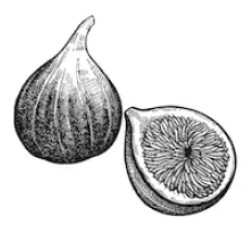
\includegraphics[width=1in,height=1.25in,clip,keepaspectratio]{fig1}}]{Michael Shell}
Use $\backslash${\tt{begin\{IEEEbiography\}}} and then for the 1st argument use $\backslash${\tt{includegraphics}} to declare and link the author photo.
Use the author name as the 3rd argument followed by the biography text.
\end{IEEEbiography}

\vspace{11pt}

\bf{If you will not include a photo:}\vspace{-33pt}
\begin{IEEEbiographynophoto}{John Doe}
Use $\backslash${\tt{begin\{IEEEbiographynophoto\}}} and the author name as the argument followed by the biography text.
\end{IEEEbiographynophoto}




\vfill




\end{document}
